
\chapter{Grundlagen}

Dieses Kapitel enth\"alt eine Einf\"uhrung in die f\"ur das Projekt eingesetzten Technologien und verwendete Hardware.

\section{Bluetooth}

Bluetooth ist eine funkbasierte Technologie f\"ur den Datenaustausch zwischen Ger\"aten auf kurzer Distanz.
Dieser Standard wurde von der \emph{Bluetooth Special Interest Group} (SIG)\cite{Bluetooth:01, Bluetooth:02} in den 90er Jahren entwickelt und
ist von dem \emph{Institute of Electrical and Electronics Engineers} (IEEE) als Standard IEEE 802.15\cite{Bluetooth:04} anerkannt.
Einsatzm\"oglichkeiten f\"ur Bluetooth sind zum Beispiel die Verbindung zwischen einem Headset und Mobiltelefon f\"ur handfreie Kommunikation 
oder Verbindung von Messger\"aten,
wie zum Beispiel einer K\"orperwaage und einem Smartphone f\"ur Protokollierung und Auswertung der Messdaten.\\


\subsection{RFCOMM}
RFCOMM steht f\"ur Radio Frequency Communication und ist ein Transportprotokoll. Es bietet vergleichbare Ausfallsicherheit, 
wie das TCP Protokoll. 
Das Ziel des RFCOMM-Protokolls ist die Emulierung einer seriellen Schnittstelle, vergleichbar der RS-232-Schnittstelle.
Dies soll den Herstellern die Anbindung ihrer Hardware, die nach diesem Standard arbeitet, erleichtern.
\cite[S. 10]{Bluetooth:03}\\

\subsection{UUID}

Verbindet sich ein Client mit einem Server, dann sucht dieser nach einem Service, den seine Anwendungsschicht verwenden m\"ochte. 
Um den entsprechenden Service zu erhalten, wird hier eine sogenannte \emph{Universally Unique Identifier} (UUID) verwendet.
Das ist ein 128-Bit-Schl\"ussel, bestehend aus hexadezimal kodierten Stellen, welcher dem Client und Server bekannt sein muss.
F\"ur die im Projekt entwickelte Software ist die UUID \emph{00001101-0000-1000-8000-00805F9B34FB} von gro\ss{}er Bedeutung.
Diese repr\"asentiert das im Projekt verwendete \emph{Serial Port Profile} (SPP). 
Dies ist notwendig, da die im Projekt eingesetzten Ger\"ate Bluetooth als serielle Schnittstelle mit diesem Profil nutzen.
\cite[S. 17]{Bluetooth:03}\\

\subsubsection{SPP}

Das Serial Port Profile ist eine Spezifikation, welche eine serielle Daten\"ubertragung \"uber Bluetooth erm\"oglicht. \\

\section{Verwendete Hardware}

F\"ur die Entwicklung der Software im Projekt wurden mehrere Ger\"ate verwendet. 
Als Basis dient ein Android-Smartphone zum Protokollieren der Messdaten.
Die Lebensmittel werden mittels einer Laborwaage gewogen und
f\"ur das Erfassen von K\"orpergewicht und Blutdruck werden entsprechende Messsensoren verwendet.
Alle Messger\"ate sind Bluetooth-f\"ahig.\\

\subsection{Android Smartphone}

Die Software wird f\"ur ein Android-Smartphone entwickelt.
Android ist ein weit verbreitetes Betriebssystem auf Smartphones und Tablets. 
Ein Android-Smartphone bringt sehr viele M\"oglichkeiten f\"ur Softwareentwickler mit sich. 
Durch die M\"oglichkeiten der Gestaltung von nahezu intuitiv bedienbaren grafischen Oberfl\"achen, profitieren die Benutzer.
Aber auch die F\"ahigkeit der Anbindung von externen Ger\"aten \"uber Schnittstellen wie Bluetooth
oder die Kommunikationsf\"ahigkeit mit dem Internet \"uber WLAN oder das Mobile Netzwerk, bieten den
Softwareentwicklern die M\"oglichkeit eine verteilte und komplexe Software mit enormen Wachstumsm\"oglichkeiten zu entwickeln.\\

\subsection{KERN PCB 6000-1 Laborwaage}

Die PCB 6000-1 ist eine hochpr\"azise Waage der Firma KERN. 
Die Abbildung 2.1 veranschaulicht das Ger\"at.
Durch ihre Genauigkeit ist sie besonders gut geeignet, um Lebensmittel in sehr kleinen aber auch gr\"o\ss{}eren Mengen zu wiegen.
Sie verf\"ugt \"uber eine RS-232-Schnittstelle, \"uber die man das gewogene Gewicht an einen Drucker oder Computer
\"ubertragen kann \cite[S. 18 - 19]{KERNPCB}.\\

\subsubsection*{Technische Daten:}

\begin{itemize}
 \item W\"agebereich [Max]: 6 kg
 \item Reproduzierbarkeit: 0.1 g
 \item Ablesbarkeit: 0.1 g
 \item Linearit\"at: 0.3 g
 \item Kleinstes Teilgewicht [Z\"ahlen]: 0.2 g/St\"uckseite
 \item Typ: PCB 6000-1
 \item Abm. Wiegeplatte: 150 x 170 mm
 \item Spannungsversorgung: 230 V/AC oder optionaler Akkupack
 \item Abm.: [L x B x H) 245 x 163 x 79 mm
 \item Besonderheit: RS-232-Schnittstelle
\end{itemize}


\begin{figure}[h]
  \centering
  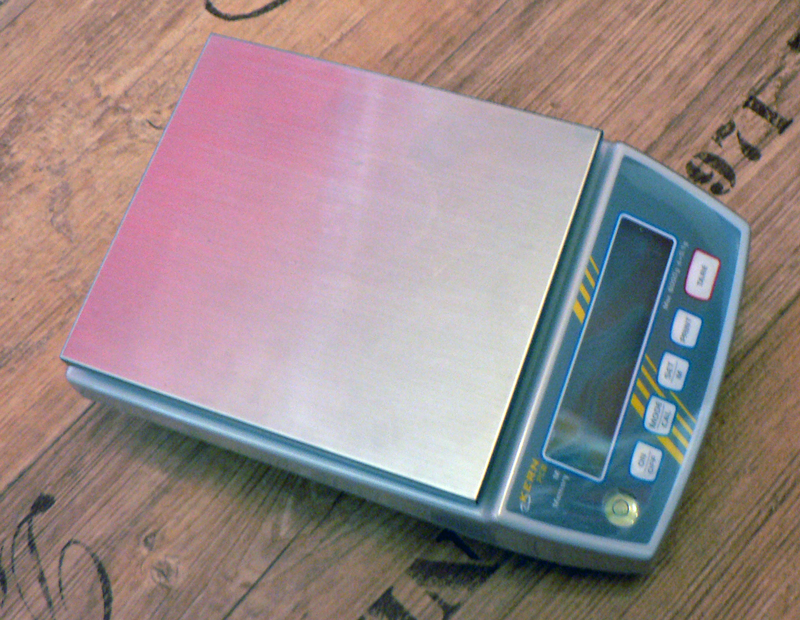
\includegraphics[scale=0.3]{fotos/devices/KERN_PCB_laborwaage.png}
  \caption{KERN PCB 6000 Laborwaage}
 
\end{figure}

\subsubsection{RS-232}

Die RS-232-Schnittstelle dient der seriellen Daten\"ubertragung. 
Es gibt sie in verschiedenen Ausf\"uhrungen.
In der Abbildung 2.2 wird die RS-232-Schnittstelle auf der R\"uckseite der PCB 6000 Waage als D-Sub-Buchse mit Adapter auf D-Sub-Stecker gezeigt.
In Verbindung mit dem Projekt wird diese Schnittstelle mit einem Bluetooth-Dongle genutzt, 
um die Wiegedaten ohne Kabel an ein Smartphone zu \"ubertragen.\\


\begin{figure}[h]
  \centering
  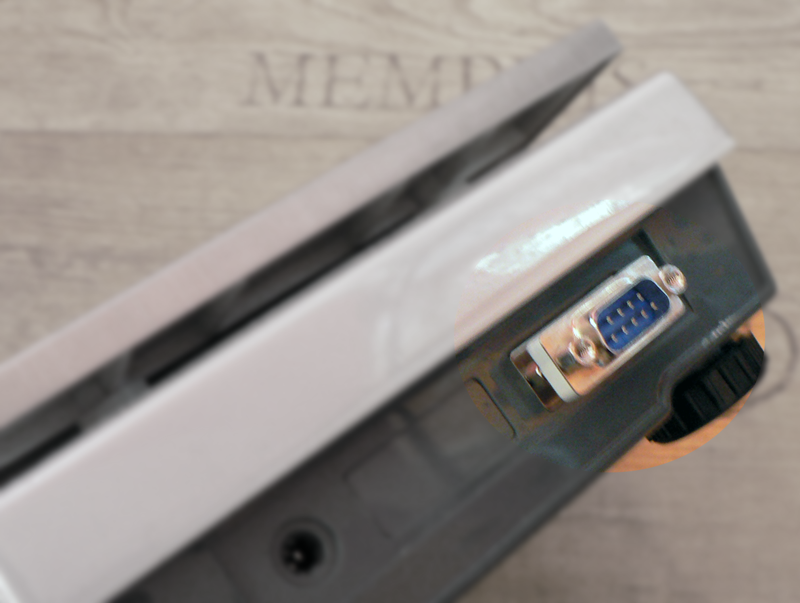
\includegraphics[scale=0.3]{fotos/devices/KERN_PCB_RS232.png}
  \caption{KERN PCB 6000 Laborwaage, R\"uckseite mit RS-232-Schnittstelle}
 
\end{figure}

\subsubsection{Bluetooth-Dongle}

Als Bluetooth-Dongle kommt das Ger\"at Pico Plug der Firma Sphinx Elektronik zum Einsatz.
Der Bluetooth-Dongle wird durch die Abbildung 2.3 veranschaulicht. 
Er erm\"oglicht eine kabellose Kommunikation zwischen zwei Ger\"aten und sendet dabei im 2,4 GHz ISM-Band.
Des Weiteren unterst\"utzt er das RFCOMM-Protokoll und SPP-Profil, welches in der Software, was sp\"ater gezeigt wird,
angewendet wird.\\

\subsubsection*{Technische Daten PICO Plug (BT-Plug)\cite{PicoPlug}:}
\begin{itemize}

  \item Ausf\"uhrung: Bluetooth-Adapter mit Microcontroller und RS-232-Schnittstelle (seriell/parallel)
  \item Protokolle: L2CAP, RFCOMM, SDP
  \item Profile: GAP, SPP, Dial-Up-Networking Profile, LAN Access Profile  
  \item Schnittstelle I: (Seriell) RS-232, Stecker D-Sub 9pol, Übertragungsgeschwindigkeit bis zu 115 kBaud
  \item Schnittstelle II: (Parallel) Centronics 36pol (Stecker), Übertragungsgeschwindigkeit 400 KBit/s
  \item Reichweite: 10 m
    
\end{itemize}
 
\begin{figure}[h]
  \centering
  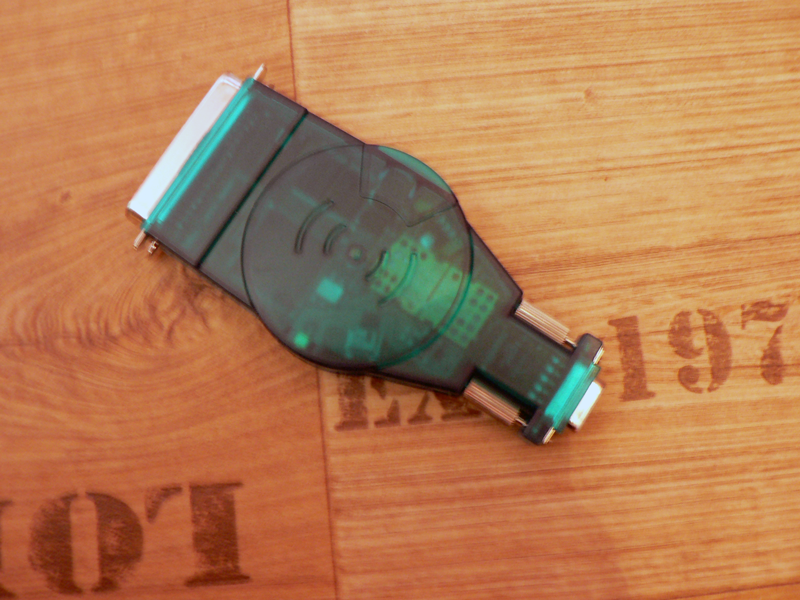
\includegraphics[scale=0.3]{fotos/devices/PicoPlug_bt_dongle.png}
  \caption{Pico Plug Bluetooth-Dongle}
 
\end{figure}

\subsection{Bodytel WeightTel}
Um das K\"orpergewicht zu erfassen, wird die K\"orperwaage WeightTel \cite{WeightTel} der Firma Bodytel eingesetzt.
Hierbei handelt es sich um eine normale elektronische K\"orperwaage ohne Zulassung als Medizinprodukt nach dem Medizinproduktgesetz.
Die Abbildung 2.4 veranschaulicht die Waage.
Dieses Ger\"at ist mit einer Bluetooth-Technologie ausgestattet und erlaubt die Messdaten an weitere Ger\"ate, wie Smartphones oder
station\"are Home-Gateways zu \"ubertragen.
Die gesendeten Daten werden in einem SMS-\"ahnlichen Format verpackt.
Auf den Aufbau und die Implementierung der SMS wird zu einem sp\"ateren Zeitpunkt n\"aher eingegangen.\\

\begin{figure}[h]
  \centering
  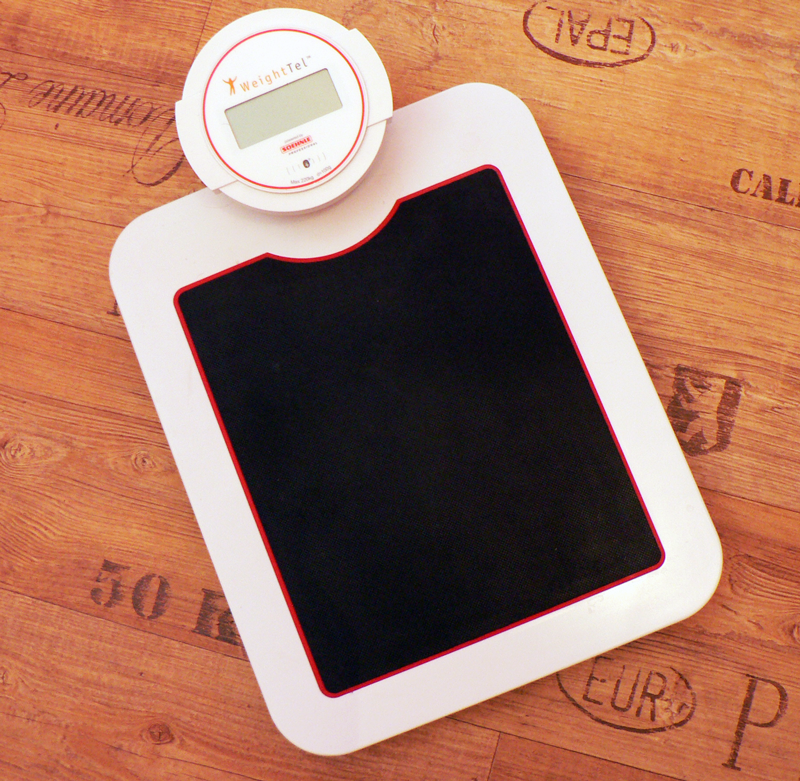
\includegraphics[scale=0.3]{fotos/devices/WeightTel_koerperwaage.png}
  \caption{Bodytel WeightTel K\"orperwaage}
 
\end{figure}

\subsubsection{Technische Daten WeightTel:\cite{WeightTel}}

\begin{itemize}
 \item Messbereich: Bis zu 220 kg
 \item Abstufung: in 100 g Schritten
 \item Trittfl\"ache: 405 x  325 mm
\end{itemize}

\subsection{Bodytel PressureTel}

F\"ur Blutdruck-Monitoring wird der PressureTel Sensor der Firma Bodytel verwendet.\cite{PressureTel} 
Dieses Produkt erf\"ullt die Medizinproduktrichtlinie 93/42/EEC \cite{med_93_42} und ist FDA 
\footnote{Food and Drug Administration: ist eine beh\"ordliche Lebensmittel\"uberwachungs- und Arzneimittelzulassungsbeh\"orde in den USA\cite{FDA:01}.} zugelassen.
Die Richtlinie dient als Instrument zum Nachweis von Sicherheit und medizinisch-technischer Leistungsf\"ahigkeit von Medizinprodukten.
Das PressureTel ist in der Lage 99 Messwerte zu speichern und diese zu einem beliebigen Zeitpunkt \"uber Bluetooth
zu Dokumentationszwecken zu \"ubertragen. 
Hierbei wird, \"ahnlich wie schon bei der K\"orperwaage, ein SMS-\"ahnliches
Format f\"ur die Datenformatierung genutzt.
Das Ger\"at PressureTel ist in der Abbildung 2.5 abgebildet.\\

\begin{figure}[h]
  \centering
  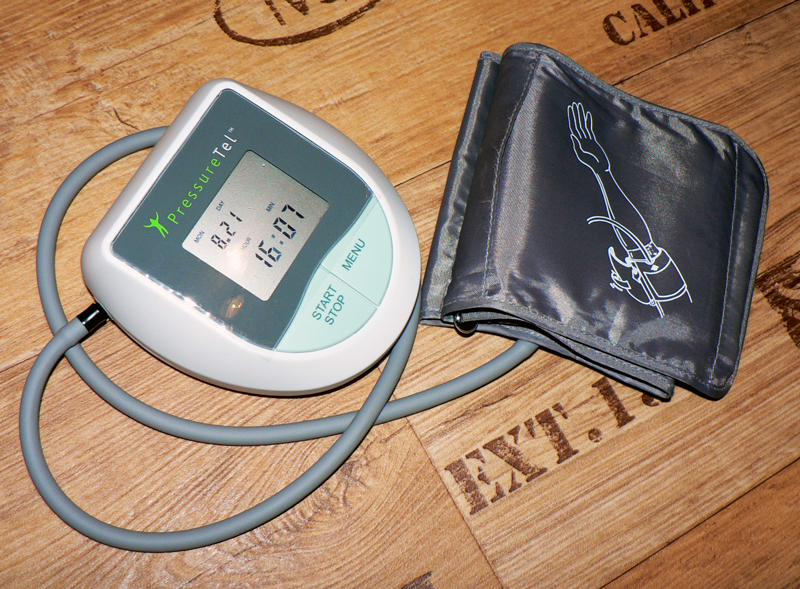
\includegraphics[scale=0.3]{fotos/devices/PressureTel_blutdruckmesser.png}
  \caption{Bodytel WeightTel K\"orperwaage}
 
\end{figure}

\subsubsection{Technische Daten:\cite{PressureTel}}

\begin{itemize}
 \item Messbereich Blutdruck:
 \subitem Systolisch: 70 bis 260 mmhg
 \subitem Diastolisch: 30 bis 180 mmHg
 \subitem Puls: 40 bis 240 Schl\"age pro Minute
 \item Druckgenauigkeit: +/- 3 mmHg
 \item Messdauer: 30 Sekunden
 \item Interface: Bluetooth
 \item Messverfahren: Oszillometrisch
\end{itemize}


\section{EAN-Barcode}

Die \emph{European Article Number\cite{EAN:01, EAN:02}} (EAN) ist eine international unverwechselbare Produktbezeichnung.
Sie ist international eindeutig und wird individuell je einem Produkt zugewiesen.
Dies wird f\"ur jedes Unternehmen von der \emph{GS1 Germany GmbH} \"ubernommen.
Man findet die EAN als Barcode im Handel auf allen Artikeln, wie zum Beispiel Lebensmitteln.
In der Regel besteht die EAN aus 13 Ziffern.
F\"ur kleine Artikel gibt es eine Ausnahme, um Platz zu sparen.
Dort ist die EAN nur 8 Ziffern lang.
Sie werden auf einer Verpackung als schwarze und wei\ss{}e Striche dargestellt.
Dabei steht Schwarz f\"ur eine 1 und Wei\ss{} f\"ur eine 0 und kodiert die EAN-Nummer bin\"ar.
Der Aufbau der EAN ist wie folgt:
\begin{itemize}
 \item Zahlen 1 bis 3 stehen f\"ur den L\"andercode. Deutschland hat den Pr\"afix 400 bis 440.
 \item Zahlen 4 bis 9 k\"onnen von der GS1 Germany einem Unternehmen nach Antrag zugeordnet werden.
 \item Zahlen 8 bis 12 werden in Abh\"angigkeit von dem Unternehmenspr\"afix von dem Unternehmen selbst f\"ur seine Artikel vergeben.
 Dabei muss die Gesamtl\"ange der EAN immer 13 Ziffern ergeben.
 \item Zahl 13 ist eine Pr\"ufziffer und dient zum Verifizieren der EAN-Nummer.
\end{itemize}

F\"ur die Produktidentifikation wird die EAN als Zahl eingegeben oder bequem mit einem Barcodescanner erfasst.
Nach Erfassen des Barcodes kann in einer Datenbank nach den Produkteigenschaften automatisch gesucht werden.
Die Abbildung 2.6 veranschaulicht ein Beispiel f\"ur einen EAN-Barcode.\\

\begin{figure}[h]
  \centering
  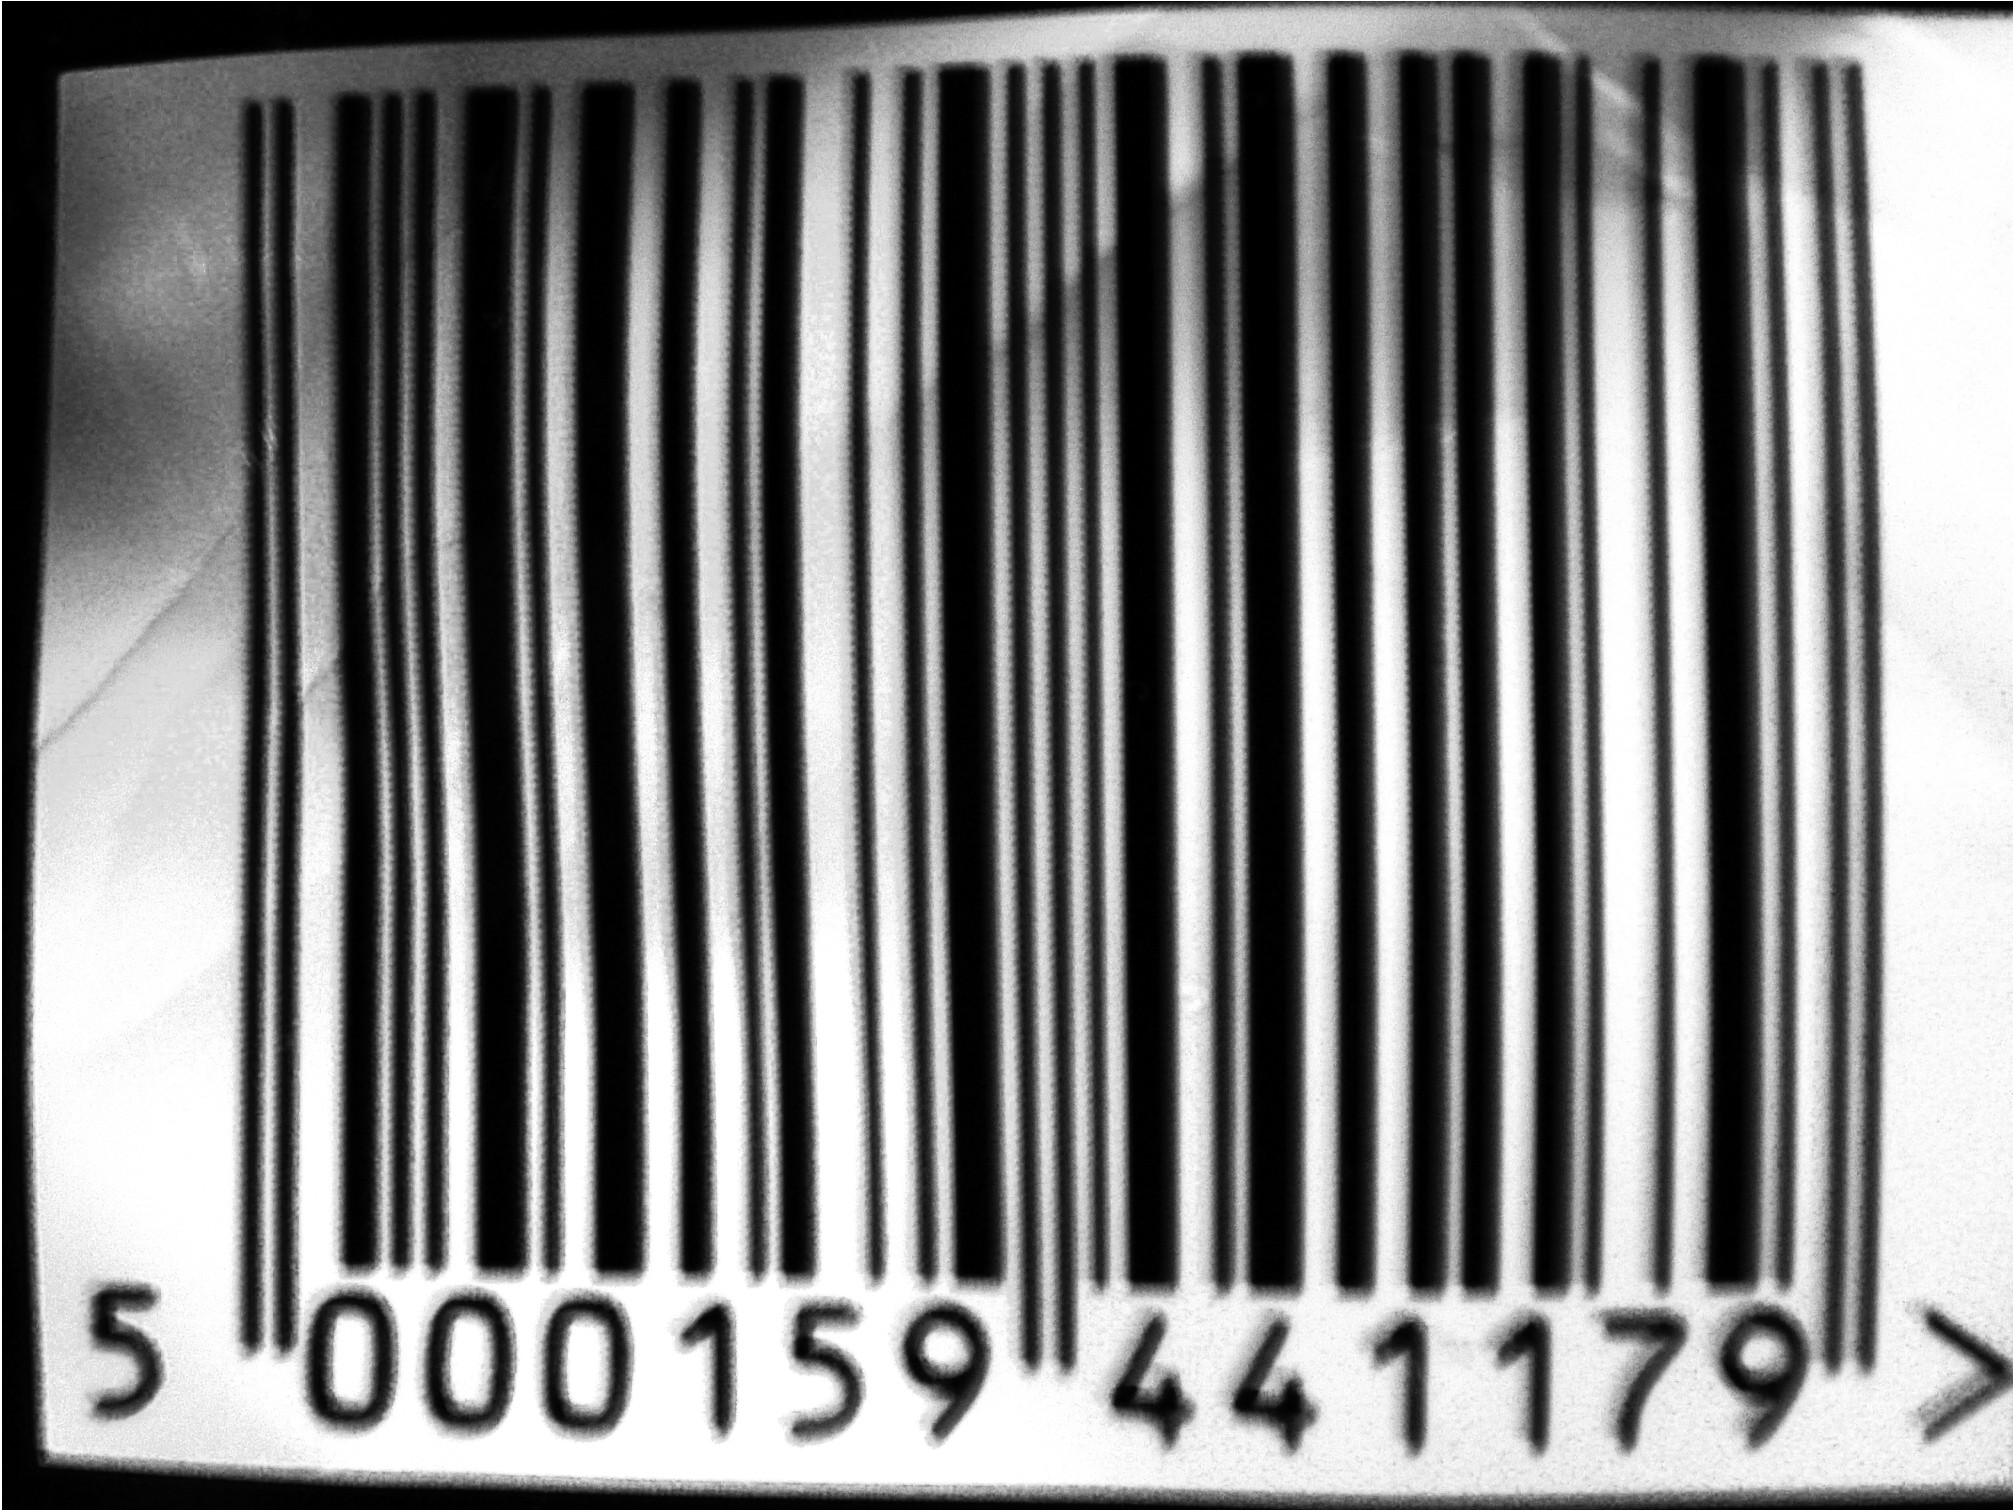
\includegraphics[scale=0.07]{fotos/extras/ean-code.jpg}
  \caption{Beispiel f\"ur ein EAN Produkt Code}
 
\end{figure}

\section{REST}

\emph{Representational State Transfer}\cite{REST:01} (REST) ist eine Architektur in der Softwareentwicklung von Webanwendungen.
Daf\"ur wird meist das zustandslose HTTP- / HTTPS-Protokoll als Transportprotokoll genutzt.
Jede Anfrage an den Server ist in sich geschlossen und der Server merkt sich keinen Zustand.
Dabei werden an eine bestimmte URL alle notwendigen Parameter \"ubergeben und die Server Software generiert eine entsprechende Antwort.
Hierf\"ur wird zum Beispiel eine weitere Anfrage an einen Datenbankserver ausgef\"uhrt. 
Die Antwort aus der Datenbank kann dann in einem beliebigen Format verpackt werden.
Meistens nutzt man daf\"ur eine XML- oder JSON-Struktur.
Sie k\"onnen aber auch als Text oder HTML-Dokument ausgegeben werden.
F\"ur die Umsetzung von REST kommt man mit den folgenden vier Methoden des HTTP-Protokolls aus: GET, POST, PUT und DELETE.\\

\begin{itemize}
 \item GET: Erlaubt das Lesen einer Ressource unter Angabe von einer URI und Parametern.
 \item POST: Erm\"oglicht ein Update von Ressourcen. Die Funktionalit\"at \"ahnelt der GET-Methode,
 allerdings k\"onnen mit der POST-Methode theoretisch unbegrenzt viele Daten an einen Server \"ubertragen werden.
 \item PUT: Dient zum Hochladen oder Erzeugen einer Ressource auf einen Server.
 \item DELETE: Erm\"oglicht das L\"oschen einer bestimmten Ressource vom Server.
\end{itemize}

Bekommt der Client eine Antwort vom Server, so kann er mit den erhaltenen Daten seine Arbeit verrichten und k\"ummert sich selbst um seinen momentanen Zustand. 
Eine Sitzungsverwaltung durch den Server ist somit nicht erforderlich.\\

In der Abbildung 2.7 wird eine m\"ogliche REST-Anfrage demonstriert.
\begin{figure}[h]
  \centering
  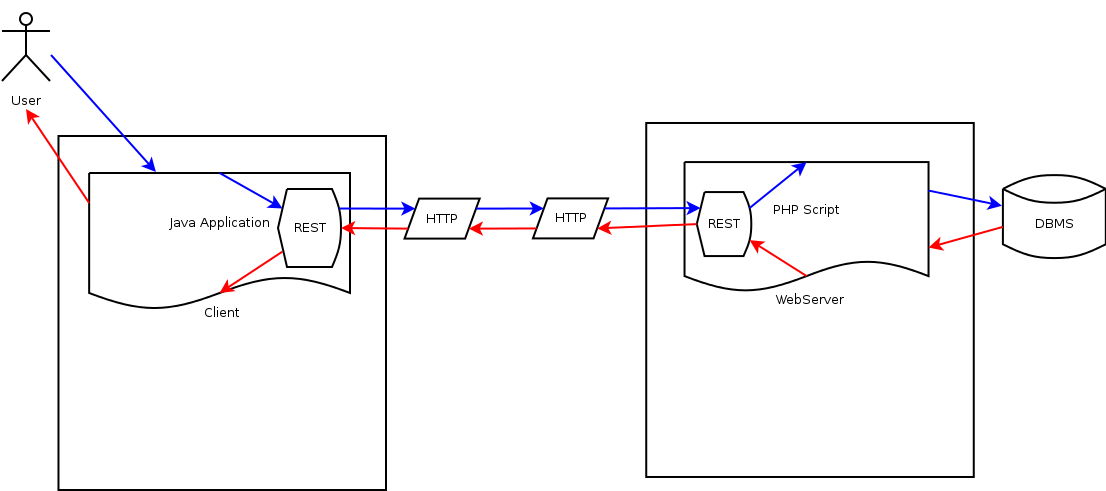
\includegraphics[scale=0.4]{diagramme/REST.png}
  \caption{Beispiel eine m\"oglichen REST-Anfrage}
 
\end{figure}

Der User startet eine Anfrage \"uber seine Anwendung.
Diese sammelt alle notwendigen Parameter und verpackt sie zum Beispiel in einen JSON-String.
Der JSON-String wird als Parameter an eine bestimmte URL \"uber HTTP gesendet.
Zum Nachverfolgen ist die Senderichtung in der Abbildung 2.7 blau gekennzeichnet.
Auf dem Server l\"auft ein PHP-Skript, welches sich um die Bearbeitung der Anfrage k\"ummert.
Das Skript extrahiert aus dem HTTP-POST oder GET den JSON-String und aus diesem die erforderlichen Parameter und verarbeitet sie.
Dazu kann zum Beispiel eine neue Anfrage an einen Datenbankserver gesendet werden.
Die Antwort aus der Datenbank wird entweder nochmal im Skript verarbeitet oder als JSON-String 
zur\"uck an den Client \"uber HTTP gesendet.
Die R\"ucksenderichtung ist hierbei rot gekennzeichnet.
Die Software auf der Client-Seite liest die Antwort des Servers aus dem JSON-String und reagiert
entsprechend darauf.\\



\section{Ajax-Architektur}

Ajax steht f\"ur \emph{Asynchronous JavaScript and XML}\cite[Kapitel 18]{Ajax:02} und stammt urspr\"unglich von Microsoft.
Es handelt sich dabei um eine Anwendungsart von bereits lange existierenden Webtechnologien wie:
HTML und CSS, DOM, JavaScript, XML und JSON und XMLHttpRequest-Objekt.
Ajax erm\"oglicht eine asynchrone Daten\"ubertragung zwischen Client und Server. 
Dabei werden Daten vom Server angefordert und in die HTML-Seite geladen, ohne, dass die Seite selbst neu geladen wird.
Der Aufbau einer solchen Kommunikation beginnt immer mit dem Erzeugen eines XMLHttpRequest-Objekts.
Das Listing 2.1 veranschaulicht diesen Vorgang mit der Unterst\"utzung f\"ur die g\"angigsten Browser.\\

\begin{lstlisting}[caption={createXHRObject() Funktion in JavaScript}]
function createXHRObject() {    
  var resObject = null;            
  try {                
    // IE 6 +
    resObject = new ActiveXObject("Microsoft.XMLHTTP");
  } catch (Error) {                
    try {
      // IE 5
      resObject = new ActiveXObject("MSXML2.XMLHTTP");
    } catch (Error) {                    
      try {
        // MOZILA, Opera, Safari ...                    
        resObject = new XMLHttpRequest();
      } catch (Error) {                    
        alert("Ajax is not supported on this browser");
      }
    }  
  }
  return resObject;
}
\end{lstlisting}

Als n\"achstes muss eine Verbindung zur Zielseite auf dem Server hergestellt werden.
Daf\"ur stellt das XHR-Objekt die Methode \emph{open()} zur Verf\"ugung. 
Sie bekommt eine URL und zwei Parameter \"ubergeben.
Die URL ist das Zieldokument, das aufgerufen wird.
Der erste Parameter entscheidet, ob die Daten \"uber POST oder GET \"ubertragen werden und der zweite Parameter 
entscheidet, ob die Methode synchron oder asynchron ausgef\"uhrt wird.
Synchron bedeutet, dass das ausf\"uhrende Skript angehalten wird bis eine Antwort vom Server zur\"uckkommt.
Im Gegensatz dazu arbeitet bei der asynchronen \"Ubertragung das Skript weiter, da die Anfrage parallel im Hintergrund ausgef\"uhrt wird.
Um auf das Ergebnis einer asynchronen Anfrage reagieren zu k\"onnen, wird eine Callback-Funktion verwendet.
Diese wird als Referenz an die Variable \emph{onreadystatechange} des XHR-Objekts \"ubergeben. 
Das Absenden der Anfrage wird \"uber die Methode \emph{send()} ausgef\"uhrt.
Wird die Anfrage als GET an den Server gesendet, so bindet man die \"Ubergabeparameter an die URL als String.
Dabei bekommt die Methode \emph{send()} beim Aufruf den Wert \emph{null} als Parameter \"ubergeben.
Wenn die Anfrage an den Server hingegen als POST gesendet wird, \"ubergibt man die Werte als Parameter an die \emph{send()} Methode.
Die Callback-Funktion wird immer aufgerufen, wenn sich der Status des XHR-Objekts \"andert.
Deshalb muss die Callback-Funktion beim Aufruf immer zuerst den Status des XHR-Objekts \"uberpr\"ufen.
Folgende Werte sind an dieser Stelle m\"oglich:
\begin{itemize}
 \item 0: nicht initialisiert
 \item 1: l\"adt
 \item 2: fertig geladen
 \item 3: wartet
 \item 4: fertig
\end{itemize}

Wird der Wert 4 ausgegeben, so kann der \emph{responseText}, also die R\"uckgabe des XHR-Objekts, ausgewertet werden.
Das Listing 2.2 veranschaulicht die Implementierung f\"ur diesen Vorgang.\\

\begin{lstlisting}[caption={Verbindungsaufbau und Callback-Funktion bei Ajax}]
function sendRequest() {  
  if (post) {
    xhr.open("post", "zielurl.php", true);
    xhr.onreadystatechange = callback;
    xhr.setRequestHeader("Content-Type", "application/x-www-form-urlencoded");
    xhr.send("a=1&b=2");
  } else if (get) {
    xhr.open("get", "zielurl.php?a=1&b=2", true);
    xhr.onreadystatechange = callback;
    xhr.send(null);
  }
}

function callback() {
  if (xhr.readyState==4) {
    //do smth...
  }
}
\end{lstlisting}

Das Anwenden von Ajax bietet viele interessante M\"oglichkeiten bei der Entwicklung von Websoftware.
Da die Daten hier immer im Klartext gesendet werden, kann es sich dabei um eine normale Textdatei,
HTML-Fragmente, XML oder JSON-Strings handeln.
Somit ist es nicht nur m\"oglich die Inhalte der sonst statischen Webseite
dynamisch zu laden, sondern es besteht auch die M\"oglichkeit die Webseite an sich im eingeschr\"ankten Umfang durch HTML-Fragmente neu zu gestalten.
Au\ss{}erdem wird die Webseite durch Ajax interaktiv und kann auf die Benutzereingaben reagieren.
Ein bekanntes Beispiel ist das Google Suggest. Diese Anwendung ist die Autovervollst\"andigung in der Eingabemaske von der Suchmaschine Google.\\

\subsection{HTML und CSS}

Die \emph{Hypertex Markup Language}\cite{HTML:01} (HTML) ist eine Auszeichnungssprache und dient zur Strukturierung von Inhalten
eines HTML-Dokuments. HTML-Dokumente dienen zur Darstellung von Text- und Bildinformationen in Webbrowsern.
Sie sind die Grundlage des \emph{World Wide Web}. Das \emph{Cascading Style Sheets}\cite{CSS:01} (CSS) ist eine deklarative Sprache und
dient der Formatierung von zum Beispiel HTML-Dokumenten.
Es erm\"oglicht nicht nur eine einfache Formatierung eines HTML-Dokuments, sondern kann auch beispielsweise bei der grafischen Oberfl\"achengestaltung 
einer QT-Anwendung (C++) genutzt werden.
In CSS3 sind einfache Animationen m\"oglich und im Rahmen eines \emph{Responsive Webdesign}\cite{RWD:01} kann man damit flexible Webseiten erstellen,
welche sich an das Ausgabeger\"at, wie zum Beispiel einen Desktop-Monitor oder ein Smartphone-Display, automatisch anpassen. \\

\subsection{DOM}
Das \emph{Document Object Model}\cite[Kapitel 3]{JavaScript:01} (DOM) ist ein Konzept einer Schnittstelle f\"ur den Zugriff auf
strukturierte Dokumente, wie HTML oder XML. 
Die Bestandteile eines HTML-Dokuments bilden dabei eine Art Baumstruktur.
Beim Laden der Webseite wird diese Struktur vom Webbrowser aufgebaut. 
Danach kann mittels JavaScript daynamisch auf die einzelnen Elemente zugegriffen werden.
Die Ideen f\"ur dieses Konzept stammen urspr\"unglich von Netscape und wurden mittlerweile in alle anderen Browser \"ubernommen.
Das folgende Listing 2.3 zeigt den HTML-Code einer Demo-Webseite. In der darauf folgenden Abbildung 2.8 wird ein Ausschnitt aus dem Ergebnisdokument im 
Webbrowser pr\"asentiert. Der dazugeh\"orige DOM-Baum wird anschlie\ss{}end in Abbildung 2.9 veranschaulicht.\\

\begin{lstlisting}[caption={Beispiel f\"ur ein einfaches HTML-Dokument}]
<html xmlns="http://www.w3.org/1999/xhtml" lang="de">
    <head>    
        <meta http-equiv="Content-Type" content="text/html; charset=utf-8" />
        <title>demo</title>
    </head>    
    
    <body>        
        <div id="knoten1">            
            <h1 id="u1"> Meine Überschrift</h1>
        </div>
        <div id="knoten2"></div>
            <p>ein Paragraph</p>
            <p>noch ein Paragraph</p>
        <div id="knoten3"></div>
    </body>
</html>

\end{lstlisting}

\begin{figure}[h]
  \centering
  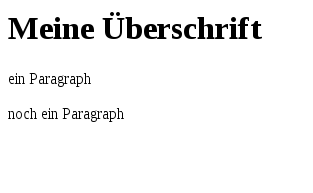
\includegraphics[scale=0.6]{fotos/kapitel2/ergebnis_html.png}
  \caption{Das Ergebnis im Browser aus dem Listing 2.3}
 
\end{figure}

\begin{figure}[h]
  \centering
  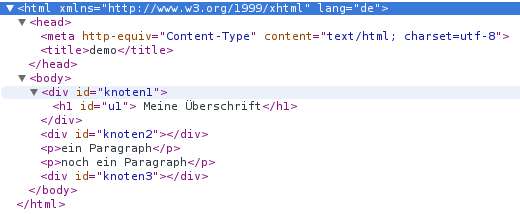
\includegraphics[scale=0.7]{fotos/kapitel2/dom_elements.png}
  \caption{Das Ergebnis des Listing 2.3 als DOM-Struktur im Webbrowser Chrome}
 
\end{figure}

Mit dem DOM-Konzept besteht die M\"oglichkeit auf Elemente im Dokument direkt zuzugreifen.
Dar\"uber hinaus hat man sogar die Option wichtige Elemente des Browsers, wie die Adressleiste, \"uber JavaScript zu manipulieren
und kann sogar neue Elemente im DOM-Baum erzeugen.
Einige wichtige Objekte aus dem DOM-Konzept sind:
\begin{itemize}
 \item document: dieses Objekt ist das zentrale Objekt moderner Programmierung. 
 Damit lassen sich neue Elemente im DOM-Baum erzeugen oder vorhandene manipulieren. 
 Es erlaubt zum Beispiel dynamisch eine Tabelle zu erzeugen oder Bilder in die Webseite zu laden.
 \item event: Steht f\"ur das Ereignis-Objekt. 
 Es ist in Browsern der verschiedenen Hersteller unterschiedlich implementiert.
 Aus diesem Grund muss man mit einer Art Browser-Weiche arbeiten, wenn man damit Events auswerten m\"ochte.
 Das k\"onnen zum Beispiel Maus-Events oder Tastatureingaben sein.
 \item form: Dar\"uber hat man Zugriff auf Formulare in einer Webseite.
 \item history: Das gibt den Zugriff auf die Historie des Browsers. 
 Im Grunde hat man den Zugriff auf den Zur\"uck-Button des Browsers.
 \item image: Das gibt den Zugriff auf alle Bilder einer Webseite.
 \item location: Mit \emph{location} hat man den Zugriff auf die Addresszeile des Besucher-Browsers.
\end{itemize}

Das Listing 2.4 demonstriert in \emph{JavaScript} eine m\"ogliche Manipulation des DOM-Baums,
der zuvor vorgestellten Demo Webseite.\\

\begin{lstlisting}[caption={Beispiel f\"ur dynamischen Zugriff auf den DOM-Baum}]

var k3 = document.getElementById("knoten3"); 
var tab = document.createElement("table");

k3.appendChild(tab);

var row1 = document.createElement("tr");
var row2 = document.createElement("tr");

for (var i = 0; i<10; i++) {

  var dat = document.createElement("td");
  dat.textContent = i;
  
  if (i%2==0)  
    row1.appendChild(dat);
    
  else  
    row2.appendChild(dat);
}

tab.appendChild(row1);
tab.appendChild(row2);
\end{lstlisting}

In der Abbildung 2.10 folgt nun das aus dem Listing 2.4 resultierende Ergebnisdokument.
Im Browser erscheinen die Ziffern 0 bis 9, je nachdem, ob sie gerade oder ungerade sind, in der oberen oder unteren Reihe. \\
Im Listing 2.4 wurde in JavaScript auf das Ergebnisdokument \"uber die Methode \emph{document.getElementById()} auf den 
\emph{knoten3} zugegriffen. 
So erh\"alt man eine Referenz auf dieses Objekt im DOM. 
Mit der Methode \emph{document.createElement()} erzeugt man weitere Objekte, welche im HTML-Code als \emph{tags} erscheinen.
Auf diese Weise wurde eine Tabelle mit zwei Reihen erzeugt.
Mit der \emph{for-Schleife} wurde die Tabelle bef\"ullt.
In der Abbildung 2.11 sieht man nun wie sich der DOM-Baum ver\"andert hat.
Der Zugriff \"uber JavaScript muss hier nicht beim Laden der Webseite geschehen. 
W\"ahrend der Benutzer die Webseite bereits betrachtet, kann eine solche Tabelle durch Interaktion zwischen Benutzer und Webseite
dynamisch nachgeladen werden.\\

\begin{figure}[h]
  \centering
  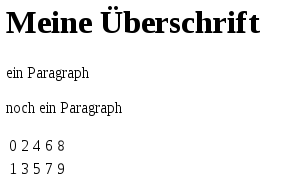
\includegraphics[scale=0.6]{fotos/kapitel2/ergebnis_html_table.png}
  \caption{Das Ergebnis im Browser aus dem Listing 2.4}
 
\end{figure}



\begin{figure}[h]
  \centering
  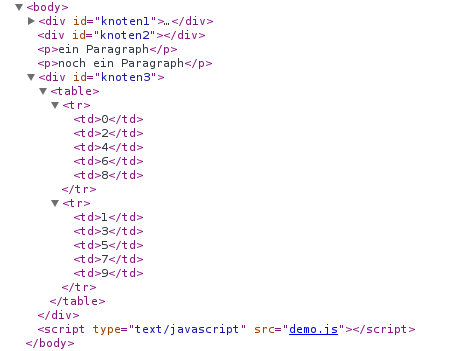
\includegraphics[scale=0.7]{fotos/kapitel2/dom_elements_table.png}
  \caption{Der DOM-Baum nach Zugriff \"uber JavaScript}
 
\end{figure}


\subsection{JavaScript}
JavaScript\cite{JavaScript:01} ist eine Skriptsprache. 
Das bedeutet, der Quellcode wird nicht kompiliert, wie das bei \emph{C/C++} der Fall ist,
sondern von einem Interpreter zur Laufzeit ausgef\"uhrt.
Ein entsprechender JavaScript-Interpreter l\"auft im Webbrowser.
Kommt der Browser beim Laden der Webseite an eine Skript-Stelle,
wie im Listing 2.5, f\"uhrt er das Skript entsprechend aus.\\

\begin{lstlisting}[caption={Eine JavaScript Datei eingebunden in ein HTML-Dokument}]
<html xmlns="http://www.w3.org/1999/xhtml" lang="de">
    <head>    
        <!-- hier ist das JavaScript eingebunden -->
        <script type="text/javascript" src="lib/js/myscript.js"></script>
    </head>        
    <body>        
       ...
    </body>
</html>

\end{lstlisting}

Wie bereits im Abschnitt der Erl\"auterung von DOM gezeigt wurde, wird JavaScript eingesetzt, um damit \"uber das DOM-Konzept
dynamisch auf die einzelnen Bestandteile einer Webseite zugreifen zu k\"onnen und diese zu manipulieren.
Das ist auch der Haupteinsatz von JavaScript. 
Des Weiteren wird JavaScript genutzt, um Eingaben in Webformularen zu \"uberpr\"ufen.
Dies geschieht direkt im Browser, noch bevor das Dokument zum Server abgeschickt wird.
Auch f\"ur Animationen auf einer Webseite oder f\"ur \emph{Rich Internet Applications} gewinnt JavaScript immer mehr an Bedeutung.
Rich Internet Applications stellen im Webbrowser Funktionalit\"at zur Verf\"ugung, wie man sie von einer Desktopanwendung kennt.
Zum Beispiel ein interaktiver Kalender oder eine Software f\"ur Textverarbeitung.
Letztendlich ist JavaScript ausschlaggebend f\"ur die Ajax-Technologie.
JavaScript erm\"oglicht das Senden und Empfangen von Daten zwischen Client und Server und
das Einbauen dieser in die Webseite. 
Dabei muss die Webseite nicht neu geladen werden.
Die Sprache ist objektbasiert und dynamisch typisiert. 
Das bedeutet, dass hier die Datentypen nicht streng verwaltet werden, wie in Java oder C++ das der Fall ist,
sondern sie ergeben sich zur Laufzeit, je nach Situation. \\


\subsection{XML und JSON}

Bei \emph{Extensible Markup Language}\cite{XML:01} (XML) handelt es sich um eine Auszeichnungssprache f\"ur eine strukturelle Darstellung von Daten im Klartext.
XML dient dem Datenaustausch zwischen Computersystemen. 
Dabei soll es aber Plattform- und Implementierungsunabh\"angig sein.
Neben dem Datenaustausch lassen sich mit XML auch Strukturen, wie der grafische Aufbau von Android \emph{Activities} umsetzen.
Das Listing 2.6 soll mit einem Beispiel f\"ur eine XML-Struktur den Aufbau verdeutlichen. 
Ein wohlgeformtes\cite{XML:02} XML-Dokument beginnt mit einem Prolog.
Dieser beinhaltet die XML-Deklaration, welche die Version, sowie den Zeichensatz angibt.
Als n\"achstes folgt das Wurzelelement, welches alle anderen Elemente umschlie\ss{}t.
In diesem Beispiel hei\ss{}t das Wurzelelement \emph{<messung>}.
Jedes Element, wie auch die Wurzel, werden mit einem \emph{tag} angek\"undigt und abgeschlossen.
Innerhalb der Wurzel k\"onnen dann beliebig viele Elemente verschachtelt werden.\\

\begin{lstlisting}[caption={Beispiel f\"ur eine Datenstruktur im XML}]
<?xml version="1.0" encoding="UTF-8"?>
<messung>
   <messart>Blutdruck</messart>
   <werte>
      <datum>2013-03-07 06:25</datum>
      <systolic>125</systolic>
      <diastolic>75</diastolic>
      <pulse>58</pulse>
   </werte>     
</messung>
\end{lstlisting}

Heute wird in Ajax kaum noch XML benutzt und wurde durch \emph{JavaScript Object Notation}\cite{JSON:01} (JSON) ersetzt.
Durch seine Struktur aus Schl\"ussel-Wert-Paaren, ist JSON ohne zus\"atzliche Mittel einfach zu lesen
und ist, wie der Name schon sagt, eine Objekt-Notation aus JavaScript.
In nahezu jeder Sprache gibt es einen JSON-Parser.
JSON kennt in seiner Notation Objekte und Arrays.
Objekte werden immer innerhalb von geschweiften Klammern und Arrays in eckigen Klammern notiert.
Objekte und Array-Elemente besitzen Eigenschaften, welche immer eindeutig sein m\"ussen.
Eine Eigenschaft besteht aus einem Schl\"ussel als Zeichenkette und einem Wert, wobei beide durch einen Doppelpunkt getrennt werden.
Im Listing 2.7 wird die gleiche Struktur aus dem Listing 2.6 als JSON veranschaulicht.
Es f\"allt auf, dass der Umfang der Notation als JSON-String, im Vergleich zu XML, geringer wird.\\


\begin{lstlisting}[caption={Beispiel aus Listing 2.6 umgesetzt in JSON}]
{
   "messart":"Blutdruck",
   "werte":{
      "datum":"2013-03-07 06:25",
      "systolic":"125",
      "diastolic":"75",
      "pulse":"58"
    }
}
\end{lstlisting}




